\documentclass{article}
\usepackage[utf8]{inputenc}

\title{%
  VarClump: A Variational Approach for Source Representation and Description \\
  \Large \textit{Applied to Astronomical Data} \\}



\author{Martín Villanueva }
\date{January 2017}

\usepackage{fourier}
    \usepackage{natbib}
\usepackage{graphicx}
\usepackage{amsmath}
\usepackage{algorithmicx}
\usepackage{algorithm}
\usepackage[noend]{algpseudocode}

\begin{document}

\maketitle



\begin{abstract}
    This work consists of ...
\end{abstract}

\section{Introduction}
There is a theory which states that if ever anyone discovers exactly what the Universe is for and why it is here, it will instantly disappear and be replaced by something even more bizarre and inexplicable.
There is another theory which states that this has already happened.


\section{Previous Work}


ClumpFind \cite{WilliamsCF} + GaussClump \cite{Stutzki} + FellWalker \cite{Berry} + Dendro \cite{Rosolowsky} (?)



\section{The VarClump Algorithm}

The proposed approach it is a multi-step algorithm composed of two main stages: 1) \textit{Continuous Fitting} and 2) \textit{Source Extraction}. The idea is to first compute an accurate continuous representation of the N-dimensional astronomical image, and then use this continuous representation to extract the clumpy structure in the data. The \textit{Continuous Fitting} step is closely related to \textit{GaussClump}, but we propose to fit a mixture of Gaussians in a globally way. The \textit{Source Extraction} is an adaptation of the \textit{Gaussian Mixture Reduction} algorithms (GMR) proposed by Williams \cite{Williams} and Runalls \cite{Runalls}.

\subsection{Variational Formulation}

Let $f_0:\mathcal{R}^N \rightarrow [0,1]$ be the N-dimensional function which represents the input data , $\alpha_1,\alpha_2 \in \mathcal{R}_0^+$ weight parameters and $\Psi_1, \Psi_2$ continuous functions that will be described later. Then we can state the problem as a minimization of the functional (\ref{eq:functional}), where $u$ is the function to find.

\begin{align}
J(u) &= \int_{\Omega \in \mathcal{R}^n} L(u, u_x, u_y, \cdots ) \\
&= \int_{\Omega \in \mathcal{R}^n} \underbrace{(u-f_0)^2}_{\text{Similarity}} + \alpha_1 \underbrace{\Psi_1(u-f)}_{\text{Restriction}} + \alpha_2 \underbrace{\Psi_2(|\nabla u|^2)}_{\text{Smoothness}} \ d\Omega
\label{eq:functional}
\end{align}

The proposed Lagrangian has three main terms described below
\begin{description}
\item \textbf{Similarity.} This is the standard terms, that ensures the similarity between data ($f$) and the continuous approximation ($u$).
\item \textbf{Restriction.} This corresponds to a problem restriction which states that no flux can be added by the function $u$, i.e, $u$ must be upper bounded by $f$. To satisfy this, $\Psi_1$ must be a positive monotone increasing function.
\item \textbf{Smoothness.} This term has two purposes: To ensure the solution will be  smooth, and to remove eventual noisy peaks in $f$.
\end{description}

Following the approach of the \textit{Calculus of Variations}, we can move from the integral formulation, to the differential formulation through the \textit{Euler-Lagrange} equation shown in (\ref{eq:eulerlagrange})
\begin{equation}
\frac{\partial L}{\partial u} - \sum_{k=1}^D \frac{d}{d x_k} \frac{\partial L}{\partial u_{x_k}} = 0 \ \ \ \text{with BC} \ \ u(\partial \Omega) = f(\partial \Omega),
\label{eq:eulerlagrange}
\end{equation}
here $D$ is the dimensionality of the problem, and Dirichlet boundary conditions were imposed.

\subsection{Penalizing Functions}

We start with $\Psi_1(x)$ since it is the more restrictive. The expected response of $\Psi_1(x)$ is not penalize at all negative inputs ($x < 0$), since in that case there is no extra flux addition from $u$. And for positive inputs ($x \geq 0$), it is expected a high and rapidly increasing penalization. With this in mind, the proposal is to use the $5$-th order spline (\ref{eq:psi})
\begin{equation}
 \widehat{\psi}(x) = \left\{
     \begin{array}{lr}
       0  & : x < 0 \\
       10 x^3 - 15 x^4 + 6 x^5 & : x \in [0,1]\\
       1 & : x >1
     \end{array}
\label{eq:psi}
\end{equation}
and then define $\Psi_1(x) = \widehat{\psi}(\lambda_1 \ x)$. In this way the parameter $\alpha_1$ controls the maximum amount of penalization, whereas $\lambda_1$ controls the speed of penalty. By construction, the spline (\ref{eq:psi}) is continuous and smooth in his entire domain. Additionally, because of his polynomial structure it is computationally cheap to evaluate it (and also his derivatives).

For the $\Psi_2(x)$ there are some standard choices like the Perona-Malik regularizer \textbf{(reference here)}. However because of the good properties exhibited by the proposal for $\Psi_1$, the same is used for $\Psi_2$, i.e, $\Psi_2(x) = \widehat{\psi}(\lambda_2 \ x)$. The parameters $\alpha_2$ and $\lambda_2$ have the same role as before.



\subsection{Solution Structure}

We parametrize the space of solutions $u$ to linear combinations of Gaussian functions as shown in (\ref{eq:mixture}). The election of Gaussian functions follows the same arguments as GaussClump \cite{Stutzki}, in addition to other advantages discussed below \textbf{(reference here)}. Each Gaussian function is described by his weight, center and covariance matrix $(c_i, \tilde{\boldsymbol{\mu}_i}, \Sigma_i)_{i=1}^N$. The value $u_0$ corresponds to the \textit{base level} of the approximation (usually set as the RMS), and is a  numerical trick to get a more stable solution.
\begin{align}
u(\mathbf{x}) &= \sum_{i=1}^N c_i \ \phi(\mathbf{x};\ \boldsymbol{\mu}_i, \boldsymbol{\theta}_i, \Sigma_{i}) + u_0 \\
&= \sum_{i=1}^N c_i \ e^{-(\mathbf{x}- \hat{\boldsymbol{\mu}_i})^T \Sigma_{i}^{-1} (\mathbf{x}-[\boldsymbol{\mu}_i + \boldsymbol{\delta} \sin(\boldsymbol{\theta}_i)]} + u_0 \\
&= \sum_{i=1}^N c_i \ e^{-(\mathbf{x}-[\boldsymbol{\mu}_i + \boldsymbol{\delta} \sin(\boldsymbol{\theta}_i)])^T \Sigma_{i}^{-1} (\mathbf{x}-[\boldsymbol{\mu}_i + \boldsymbol{\delta} \sin(\boldsymbol{\theta}_i)]} + u_0.
\label{eq:mixture}
\end{align}

In order to get a meaningful and simple model, the following restrictions are imposed over $u$:
\begin{enumerate}
    \item The weights $c_i$ should be always in $\mathcal{R}^+$.
    \item The center of Gaussians are restricted to be in the interior domain $\Omega - \partial \Omega$. To satisfy that, we introduce the \textit{reference centers} $\boldsymbol{\mu}_i$, the neighborhood ratio $\boldsymbol{\delta} \in \mathcal{R}^D$ and a control parameter $\boldsymbol{\theta}_i \in \mathcal{R}^D$. Then the actual centers of each Gaussian are computed as $\tilde{\boldsymbol{\mu}_i} = \boldsymbol{\mu}_i + \boldsymbol{\delta} \sin(\boldsymbol{\theta}_i)$ (here, $sin$ is applied element-wise).
    \item The Gaussians are spherically symmetrical, i.e, $\Sigma_i$ is a diagonal matrix with the same value $\sigma_i$ in the diagonal. Additionally we introduce the \textit{minimal broadening} $\sigma_0$ parameters, which is the minimal width that a Gaussian can have. The structure of the covariance matrix is shown below.
    \begin{equation*}
     \Sigma_i = 
     \begin{pmatrix}
     \sigma_i + \sigma_0 & 0 & 0 \\
     0 & \sigma_i + \sigma_0 & 0 \\
     0 & 0 & \sigma_i + \sigma_0
     \end{pmatrix}
    \label{eq:sigma}
    \end{equation*}
\end{enumerate}

The first two restrictions are needed to ensure physical/astronomical sense. The third is for simplicity in the optimization step (Section \ref{optimization}). It is also possible to extend $\Sigma_i$ to have elliptical symmetry and orientation. The trade-off between model complexity and optimization cost is discussed in Section \label{future}.

Replacing equation (\ref{eq:mixture}) into (\ref{eq:eulerlagrange}) we get a nonlinear system of equations. In order to simplify the optimization problem, we choose the \textit{reference centers} $\boldsymbol{\mu}_i$ with one of the methods presented in Section \ref{centers} and the neighborhood ratio $\boldsymbol{\delta}$ is equal for all Gaussians and set according to the problem properties. Given that, for each Gaussian the parameters to be found are $(\boldsymbol{\theta}_i, c_i, \sigma_i)_{i=1}^N$ ($D+2$ parameters for each one), and we need to evaluate the Euler-Lagrange equation on (at least) $(D+2)\cdot N$ points to have a consistent system of nonlinear equations.


\subsection{Centers Generation} \label{centers}

It is necessary to introduce the two sets of points that we will be using, the \textbf{center points} $\mathcal{P}$ corresponding to the center of Gaussians introduced above, and \textbf{collocation points} $\mathcal{Q}$ which are the points where the Euler-Lagrange equation will be evaluated. Both set of points will be generated with the method described in this section.

Additionally there are two necessary conditions that the points $\mathcal{P}$ and $\mathcal{Q}$ should satisfy.
\begin{enumerate}
\item \textit{Center points should be concentrated at high intensity zones}. High intensity zones are most probably where clumps/sources are located, so clusterizing the centers around them give us enough capacity such clump/source well.
\item \textit{Collocation points should contain center points}: $P \subset Q$. To understand this point consider the situation in Figure \ref{fig:example}. If we try to fit a Gaussian function centered at the center point (red), which is between to collocation points (green), two situations can occur:
\begin{enumerate}
\item If $\sigma^2$ is small then $c$ will be huge, and as a result we get a singular/high intensity Gaussian.
\item If $c$ is small then $\sigma^2$ will be huge, adding flux/noise to the whole approximation $u$.
\end{enumerate}
\end{enumerate}

\begin{figure}[htpb!]
\centering
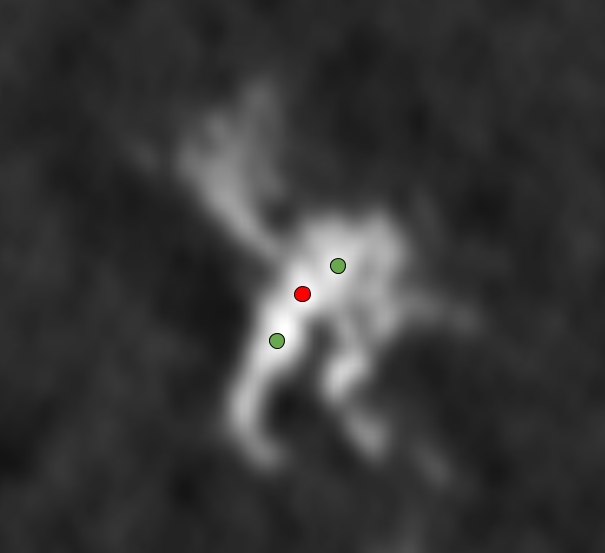
\includegraphics[width=8cm]{vc_img_00}
\caption{Example for necessary condition 2. Center point in red. Collocation points in green.}
\label{fig:example}
\end{figure}

The proposed method is based on treating the data $f_0$ as an \textit{empirical random distribution}, which will be sampled to get the sets $\mathcal{P}$ and $\mathcal{Q}$. For that, instead of $f_0$ we will use $F_0$, the original N-dimensional data cube scaled in the range $[0,1]$. The full algorithm is described in \ref{alg:centers}. Some details must be noted:
\begin{itemize}
\item We introduce a parameter \texttt{pow}, which is the power to be applied on $F_0$ to create the probability matrix $P$.
\item The sampling is repeated $2*|\mathcal{P}|$ times. The first $|\mathcal{P}|$ points are assigned to $\mathcal{P}$, and all the selected points are assigned to $\mathcal{Q}$. In this way we ensure the second necessary condition stated above.
\item A kernel matrix $K$ is multiplied in the neighborhood of the selected pixel in $P$, setting to $0$ the probability of the current selected pixel and decreasing the probability of the neighbor pixels.
\end{itemize}

\begin{algorithm}
\caption{Centers generator through random sampling $F_0$}\label{alg:centers}
\begin{algorithmic}[1]
\Procedure{\texttt{center\_generator}}{$F_0$, \texttt{n\_center}, \texttt{pow}}
\State{$F_0$ = $F_0^{\texttt{pow}}$}
\State{$P$ = $F_0/\texttt{sum}(F_0)$}
\State{\texttt{selected\_pixels} = \texttt{list()}}
\While{\texttt{len(selected\_pixels) != $2 \cdot \texttt{n\_center}$}}
\State{\texttt{pixel\_position = } \texttt{sample}($P$)}
\State{\texttt{selected\_pixels.append( pixel\_position )}}
\State{$P[\texttt{pixel\_position} \pm \delta]$ \texttt{*=} $K$}
\State{$P$ = $P/\texttt{sum}(P)$}
\EndWhile
\EndProcedure
\end{algorithmic}
\end{algorithm}




\subsection{Optimization} \label{optimization}

Iterative approach v/s LM approach





\section{Experiments} \label{experiments}



\section{Enhancements and Future Work} \label{future}



\section{Conclusions} \label{conclusions}




``I always thought something was fundamentally wrong with the universe'' \citep{adams1995hitchhiker}

\bibliographystyle{unsrt}
\bibliography{references}
\end{document}
